% !TEX program = xelatex
% Compile from this directory: xelatex -no-shell-escape TenSyGrid_WP4_Plenary_November_2026.tex
% Run twice to update navigation and PDF metadata.
%
% DRAFT: WP4 update for the November 2026 plenary.
% Reporting period: since the Malta plenary, November 2025.
% Target: approximately 20 minutes; no live GUI demo.
% The hackathon runs concurrently with the plenary: do not report outcomes.
%
% TO CONFIRM BEFORE PRESENTING (kept out of the projected slides):
% 1. Exact plenary date: source slides contain conflicting dates. Month only below.
% 2. What was already presented in Malta; overview describes current outputs,
%    without assigning an unverified completion date to each feature.
% 3. Latest tested networks, reference comparisons and performance measurements.
%    Do not describe IEEE-25 / IEEE-118 as validated without supporting results.
% 4. Formal D4.1 / MS4.1 submission and approval status. The supplied D4.1 has
%    future approval/submission dates; MS4.1 still records review pending.
% 5. Final hackathon rules and scoring: intentionally omitted here.
%
% SOURCES (paths relative to this package):
% ../D-4.1-v2.2.0.pdf: printed pp. 9-19, 20-30 and 43.
% ../MS4.1-TenSyGrid-UPC.pdf: pp. 4-6, including the generator-outage example.
% ../Plenary_November_26_TenSyGrid_WP4.pptx.pdf: authors and task headings.
% Extracted screenshots retain their original values. They show separate runs.

\documentclass[aspectratio=1609,9pt]{beamer}
\usepackage[english]{babel}
\usepackage[UPC]{tensygrid}
\usepackage{mathtools}
\usepackage{tikz}
\usetikzlibrary{calc,arrows.meta}
\usepackage{pgfgantt}

\definecolor{wpblue}{HTML}{1B587C}
\definecolor{taskpurple}{HTML}{9E2A8F}
\definecolor{highlightred}{HTML}{FF0000}

% Configuration is loaded lowercase, whereas the supplied logo is UPC-logo.pdf.
% Restore its case for the existing footer after the configuration is loaded.
\makeatletter
\def\TG@config{UPC}
\makeatother
% Use the template's original logo files in its two-row acknowledgement layout.
\newcommand{\compactfundinglogos}{%
  \begin{center}
    
\includegraphics[height=14mm]{config/CETP-logo.pdf}\hspace{12mm}%
    
\includegraphics[height=16mm]{config/EU-logo.pdf}\\[5mm]
    
\includegraphics[width=.12\linewidth,height=18mm,keepaspectratio]{config/BMWE-logo.pdf}\hfill
    
\includegraphics[width=.24\linewidth,height=18mm,keepaspectratio]{config/MCIU-logo.pdf}\hfill
    
\includegraphics[width=.16\linewidth,height=18mm,keepaspectratio]{config/AEI-logo.pdf}\hfill
    
\includegraphics[width=.12\linewidth,height=18mm,keepaspectratio]{config/CDTI-logo.pdf}\hfill
    
\includegraphics[width=.15\linewidth,height=18mm,keepaspectratio]{config/XJENZA-logo.pdf}
  \end{center}}
\setbeamertemplate{navigation symbols}{}

\author[UPC -- CITCEA]{\texorpdfstring{Eduardo Prieto-Araujo\\Alexandre Gràcia Calvo\\Carlos Herrera Vázquez}{Eduardo Prieto-Araujo; Alexandre Gràcia Calvo; Carlos Herrera Vázquez}}
\title[WP4 -- TenSyGrid Toolbox]{WP4 updates}
\subtitle{TenSyGrid Toolbox Development}
\date[Nov 2026]{Plenary meeting -- November 2026}
\hypersetup{pdfauthor={Eduardo Prieto-Araujo; Alexandre Gràcia Calvo; Carlos Herrera Vázquez},
  pdftitle={TenSyGrid WP4 -- November 2026 plenary}}

\begin{document}

% 1 -- 0:30. Reporting period confirmed by Alexandre.
\begingroup
\setbeamertemplate{footline}{}
\begin{frame}
  \titlepage
\end{frame}
\endgroup

% 2 -- 2:00. Current documented outputs; not a verified feature-by-feature delta.
% Sources: D4.1 summary and conclusions; MS4.1 p. 4.
\begin{frame}[t]{WP4 progress since Malta}
  \framesubtitle{November 2025 -- November 2026}
  \vspace{1.5ex}
  \begin{itemize}\setlength{\itemsep}{2ex}
    \item \textbf{T4.1 -- Use cases:} a structured catalogue informed by industry interviews and prototype development.
    \item \textbf{T4.2 -- Analysis methods:} multilinear stability analysis within the VeraGrid-based workflow.
    \item \textbf{T4.3--T4.4 -- Implementation:} five core use cases functional in the Stability Monitor prototype.
  \end{itemize}
  \vfill
  {\color{tgpetrol}\textbf{Current focus:} consolidate the working core and select the next extensions.}
\end{frame}

% 2b -- WP4 progress timeline (Gantt chart).
\begin{frame}[t]{WP4 progress -- Timeline}
  \vspace{2ex}
  \centering
  \resizebox{\textwidth}{!}{%
    \begin{ganttchart}[
        x unit=0.38cm,
        y unit title=0.55cm,
        y unit chart=0.6cm,
        hgrid=false,
        vgrid=false,
        canvas/.style={draw=none},
        title/.style={draw=none, fill=none},
        title label font=\sffamily\scriptsize\bfseries,
        title height=1,
        bar height=1,
        bar/.style={draw=none},
        bar label font=\sffamily\scriptsize,
        bar label text={},
        include title in canvas=false
      ]{1}{36}
      % Month numbers header row (space reserved)
      \gantttitle{}{36} \\

      % Tasks (bars via pgfgantt)
      \ganttbar[name=wp4, bar/.append style={fill=wpblue}]{}{6}{36} \\
      \ganttbar[name=t41, bar/.append style={fill=taskpurple}]{}{6}{12} \\
      \ganttbar[name=t42, bar/.append style={fill=taskpurple}]{}{12}{24} \\
      \ganttbar[name=t43, bar/.append style={fill=taskpurple}]{}{10}{27} \\
      \ganttbar[name=t44, bar/.append style={fill=taskpurple}]{}{10}{36}

      % Custom overlays: lines, labels, and current status indicator
      \begin{scope}[line width=0.4pt, black]
        % Key positions (1 month = 0.38cm). wp4 starts at month 6.
        \coordinate (m1L)  at ($(wp4.west |- wp4.north) + (-5*0.38cm, 0.55cm)$); % before month 1, top of header
        \coordinate (m1Lb) at ($(wp4.west |- t44.south) + (-5*0.38cm, 0)$);       % before month 1, bottom
        \coordinate (m13L) at ($(wp4.west |- wp4.north) + (7*0.38cm, 0.55cm)$);   % between 12-13, top
        \coordinate (m13b) at ($(wp4.west |- t44.south) + (7*0.38cm, 0)$);
        \coordinate (m25L) at ($(wp4.west |- wp4.north) + (19*0.38cm, 0.55cm)$);  % between 24-25, top
        \coordinate (m25b) at ($(wp4.west |- t44.south) + (19*0.38cm, 0)$);
        \coordinate (hdrTR) at ($(wp4.east |- wp4.north) + (0, 0.55cm)$);          % header top-right (month 36 end)
        \coordinate (hdrBR) at (wp4.east |- wp4.north);                            % header bottom-right
        \coordinate (hdrTL) at ($(wp4.west |- wp4.north) + (-7.2cm, 0.55cm)$);     % header top-left (label area)
        \coordinate (hdrBL) at ($(wp4.west |- wp4.north) + (-7.2cm, 0)$);          % header bottom-left

        % Header horizontal lines (above and below header row: Nº, Title, 1..36)
        \draw (hdrTL) -- (hdrTR);
        \draw (hdrBL) -- (hdrBR);

        % Year separators: before month 1, between 12-13, between 24-25
        \draw (m1L) -- (m1Lb);
        \draw (m13L) -- (m13b);
        \draw (m25L) -- (m25b);
      \end{scope}

      % "Month" label above month 1 and header/row labels, consistently aligned
      \node[font=\sffamily\scriptsize\bfseries, anchor=south west]
      at ($(wp4.west |- wp4.north) + (-5*0.38cm, 0.62cm)$) {Month};
      \node[font=\sffamily\scriptsize\bfseries, anchor=east, align=left, text width=7.2cm, inner xsep=0pt]
      at ($(wp4.west |- wp4.north) + (0, 0.24cm)$) {\makebox[0.6cm][l]{Nº}\hspace{0.2cm}\parbox[c]{4.4cm}{Title}};
      \foreach \m in {1,...,36} {
          \node[font=\sffamily\scriptsize\bfseries, anchor=center]
          at ($(wp4.west |- wp4.north) + ({(-5.5+\m)*0.38cm}, 0.24cm)$) {\m};
        }

      \node[font=\sffamily\scriptsize\bfseries, anchor=east, align=left, text width=7.2cm, inner xsep=0pt]
      at (wp4.west |- wp4.center) {\makebox[0.6cm][l]{WP4}\hspace{0.2cm}\parbox[t]{4.4cm}{TenSyGrid Toolbox Development $\rightarrow$}};
      \node[font=\sffamily\scriptsize, anchor=east, align=left, text width=7.2cm, inner xsep=0pt]
      at (wp4.west |- t41.center) {\makebox[0.6cm][l]{T4.1}\hspace{0.2cm}\parbox[t]{4.4cm}{Identification of Use-cases}};
      \node[font=\sffamily\scriptsize, anchor=east, align=left, text width=7.2cm, inner xsep=0pt]
      at (wp4.west |- t42.center) {\makebox[0.6cm][l]{T4.2}\hspace{0.2cm}\parbox[t]{4.4cm}{Multilinear tools for power system stability analysis}};
      \node[font=\sffamily\scriptsize, anchor=east, align=left, text width=7.2cm, inner xsep=0pt]
      at (wp4.west |- t43.center) {\makebox[0.6cm][l]{T4.3}\hspace{0.2cm}\parbox[t]{4.4cm}{Toolbox framework development and implementation}};
      \node[font=\sffamily\scriptsize, anchor=east, align=left, text width=7.2cm, inner xsep=0pt]
      at (wp4.west |- t44.center) {\makebox[0.6cm][l]{T4.4}\hspace{0.2cm}\parbox[t]{4.4cm}{Network analysis applications}};

      % Current status indicator: month 23 column (WP4 to T4.4) and arrow above 23
      \coordinate (m23L) at ($(wp4.west |- wp4.north) + (17*0.38cm, 0)$);
      \coordinate (m23R) at ($(wp4.west |- wp4.north) + (18*0.38cm, 0)$);
      \coordinate (m23Lb) at ($(m23L |- t44.south)$);
      \coordinate (m23Rb) at ($(m23R |- t44.south)$);
      \draw[highlightred, line width=1.2pt] (m23L) rectangle (m23Rb);

      \coordinate (m23Top) at ($(m23L)!0.5!(m23R) + (0,0.55cm)$);
      \fill[highlightred]
      ($(m23Top) + (0,0.08cm)$) --
      ($(m23Top) + (-0.11cm,0.30cm)$) --
      ($(m23Top) + (0.11cm,0.30cm)$) -- cycle;
    \end{ganttchart}%
  }
\end{frame}

% 3 -- 2:30. Sources: D4.1 sections 2.3, 3.1 and 4; MS4.1 p. 4.
% Stakeholder interviews validate relevance, not numerical model accuracy.
\begin{frame}[t]{T4.1 -- Use-case catalogue}
  \framesubtitle{14 documented cases: 5 implemented, 9 proposed}
  \vspace{1ex}
  \begin{columns}[T,onlytextwidth]
    \begin{column}{0.44\textwidth}
      {\color{tgpetrol}\textbf{Implemented -- Stability Monitor}}
      \small
      \begin{itemize}\setlength{\itemsep}{1.1ex}
        \item \textbf{UC-01} -- Small-signal stability analysis.
        \item \textbf{UC-02} -- Stability-margin screening and eigenvalue monitoring.
        \item \textbf{UC-03} -- Critical oscillatory-mode diagnosis.
        \item \textbf{UC-04} -- Bus-voltage profiles and limit violations.
        \item \textbf{UC-05} -- Stability risks under $N-1$ contingencies.
      \end{itemize}
    \end{column}
    \begin{column}{0.53\textwidth}
      {\color{tgpetrol}\textbf{Proposed extensions}}
      \small
      \begin{itemize}\setlength{\itemsep}{0.5ex}
        \item \textbf{UC-06} -- Operating-scenario comparison.
        \item \textbf{UC-07} -- Device contributions to stability issues.
        \item \textbf{UC-08} -- Stability margins as loading increases.
        \item \textbf{UC-09} -- Critical system-element ranking.
        \item \textbf{UC-10} -- Damping-controller placement.
        \item \textbf{UC-11} -- Renewable-integration impact on stability.
        \item \textbf{UC-12} -- Automated documentation and reporting.
        \item \textbf{UC-13} -- Nonlinear behaviour near critical points.
        \item \textbf{UC-14} -- Region of attraction after disturbances.
      \end{itemize}
    \end{column}
  \end{columns}
  \vfill
  %{\scriptsize Source: D4.1, use-case catalogue. UC-13 and UC-14 are research-oriented proposals.}
\end{frame}

% 4 -- 3:00. Source: D4.1 sections 2.2 and 3.2.1.
% Explain equilibrium and local linearization. Do not claim a measured speed-up
% or describe local small-signal analysis as a large-disturbance certificate.
\begin{frame}[t]{T4.2 -- Multilinear stability analysis}
  \vspace{1ex}
  \begin{itemize}\setlength{\itemsep}{1.5ex}
    \item Multilinear component models support system assembly and linearization at the operating point.
    \item The resulting descriptor model is used for small-signal analysis:
  \end{itemize}
  \vspace{0.5ex}
  \[
    \mathbf{E}\Delta\dot{\mathbf{x}}=\mathbf{A}\Delta \mathbf{x},
    \qquad \mathbf{A} \mathbf{v}_k=\lambda_k \mathbf{E} \mathbf{v}_k
  \]
  \vspace{0.5ex}
  \begin{itemize}\setlength{\itemsep}{1.5ex}
    \item Outputs: eigenvalues, oscillation frequencies, damping ratios and participation factors.
    \item These results support system screening, mode diagnosis and contingency comparison.
  \end{itemize}
\end{frame}

% 5 -- 2:00. Simplified from D4.1 Figure 2.2 (fig:tool_pipeline),
% deliverable/Chapters/methodology_architecture.tex.
% Do not imply every external format includes complete, validated dynamic data.
\begin{frame}[t]{T4.3 -- Integrated toolbox workflow}
  \framesubtitle{Native Python implementation built on VeraGrid}
  \vspace{0.5ex}
  \centering
  \begin{tikzpicture}[
    stage/.style={draw=tgpetrol, line width=0.6pt,
        text width=12cm, minimum height=0.8cm, inner sep=3pt,
        align=center, font=\small},
    flow/.style={-{Latex[length=1.8mm]}, draw=tgpetrol, line width=0.8pt},
    transfer/.style={font=\scriptsize, fill=white, inner sep=1pt}
    ]
    \node[stage, fill=green!12] (ingest) at (0,0) {
      \textbf{1. Model ingestion -- VeraGrid imports / IPSA / API}\\
      Network topology, equipment parameters and required dynamic models
    };
    \node[stage, fill=yellow!18] (operating) at (0,-1.25) {
      \textbf{2. Operating point -- VeraGridEngine}\\
      Grid modeling and AC/DC power flow
    };
    \node[stage, fill=yellow!18] (analysis) at (0,-2.5) {
      \textbf{3. Stability analysis -- TenSyGridEngine}\\
      Descriptor assembly, modal analysis and $N-1$ screening
    };
    \node[stage, fill=cyan!10] (monitor) at (0,-3.75) {
      \textbf{4. Result inspection -- Stability Monitor (web)}\\
      System status, critical modes, voltage profiles and contingency comparison
    };
    \draw[flow] (ingest.south) -- (operating.north)
    node[midway, right=2mm, transfer] {Validated \texttt{MultiCircuit} model};
    \draw[flow] (operating.south) -- (analysis.north)
    node[midway, right=2mm, transfer] {Equilibrium $\mathbf{x}_0$ and implicit equations};
    \draw[flow] (analysis.south) -- (monitor.north)
    node[midway, right=2mm, transfer] {Eigenvalues, damping, participation and contingencies};
  \end{tikzpicture}
  \par\vspace{0.6ex}
  %{\scriptsize Adapted from D4.1, Fig.\ 2.2. Inputs must include the dynamic data required by the analysis.}
\end{frame}

% 6 -- 3:30. Source: D4.1 UC-01 to UC-05; screenshot from PDF page 25,
% printed p. 24, Figure 3.4. This is a different run from the next slide.
\begin{frame}[t]{T4.4 -- Five implemented use cases}
  \vspace{1ex}
  \begin{columns}[T,onlytextwidth]
    \begin{column}{0.43\textwidth}
      \begin{itemize}\setlength{\itemsep}{1.5ex}
        \item \textbf{UC-01} -- Run small-signal analysis.
        \item \textbf{UC-02} -- Screen system status and eigenvalues.
        \item \textbf{UC-03} -- Diagnose critical modes.
        \item \textbf{UC-04} -- Check bus-voltage profiles.
        \item \textbf{UC-05} -- Assess N$-$1 contingencies.
      \end{itemize}
    \end{column}
    \begin{column}{0.54\textwidth}
      \centering
      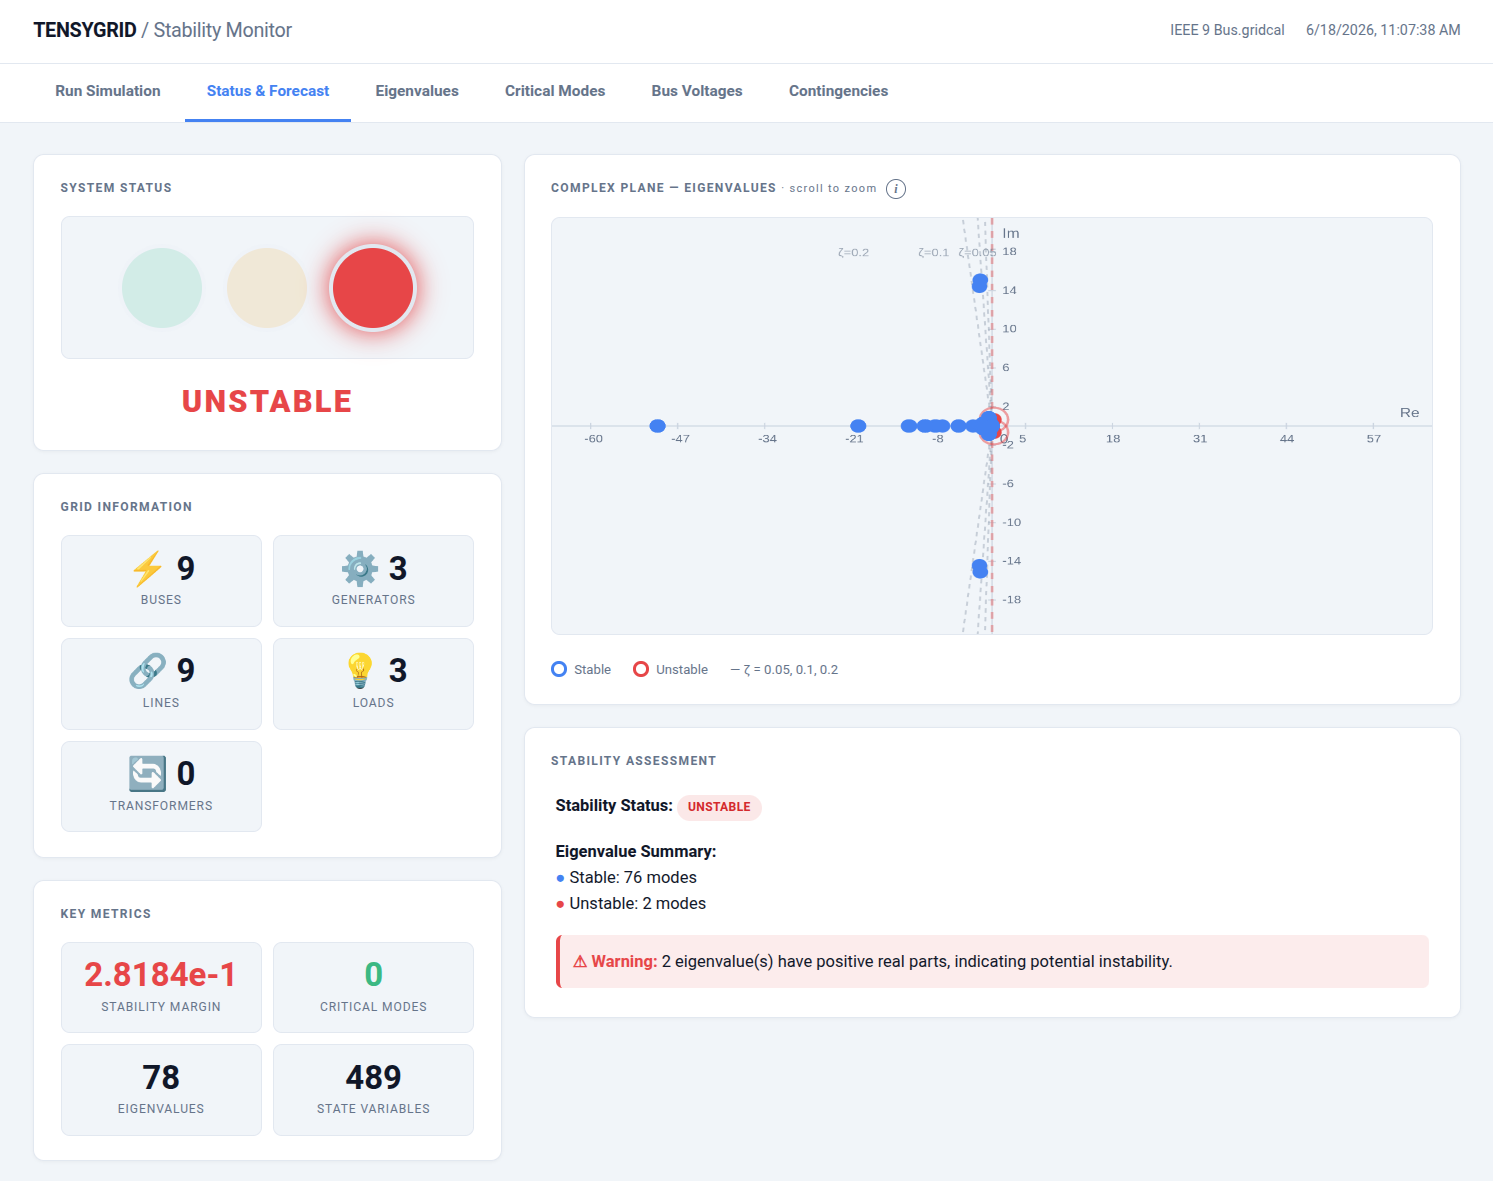
\includegraphics[width=\linewidth,height=0.55\paperheight,keepaspectratio]{assets/stability-status.png}\\[0.5ex]
      {\scriptsize Stability Monitor: system status and eigenvalue screening.\\Source: D4.1, Fig. 3.4; illustrative prototype run.}
    \end{column}
  \end{columns}
\end{frame}

% 7 -- 3:30. Source: MS4.1 p. 6, Figure 3.
% The caption identifies an IEEE 9-bus EMT multilinear example.
% This result illustrates the workflow, not validation across all networks.
\begin{frame}[t]{Example -- Generator outage}
  \framesubtitle{IEEE 9-bus EMT multilinear model}
  \vspace{0.5ex}
  \begin{columns}[T,onlytextwidth]
    \begin{column}{0.59\textwidth}
      \centering
      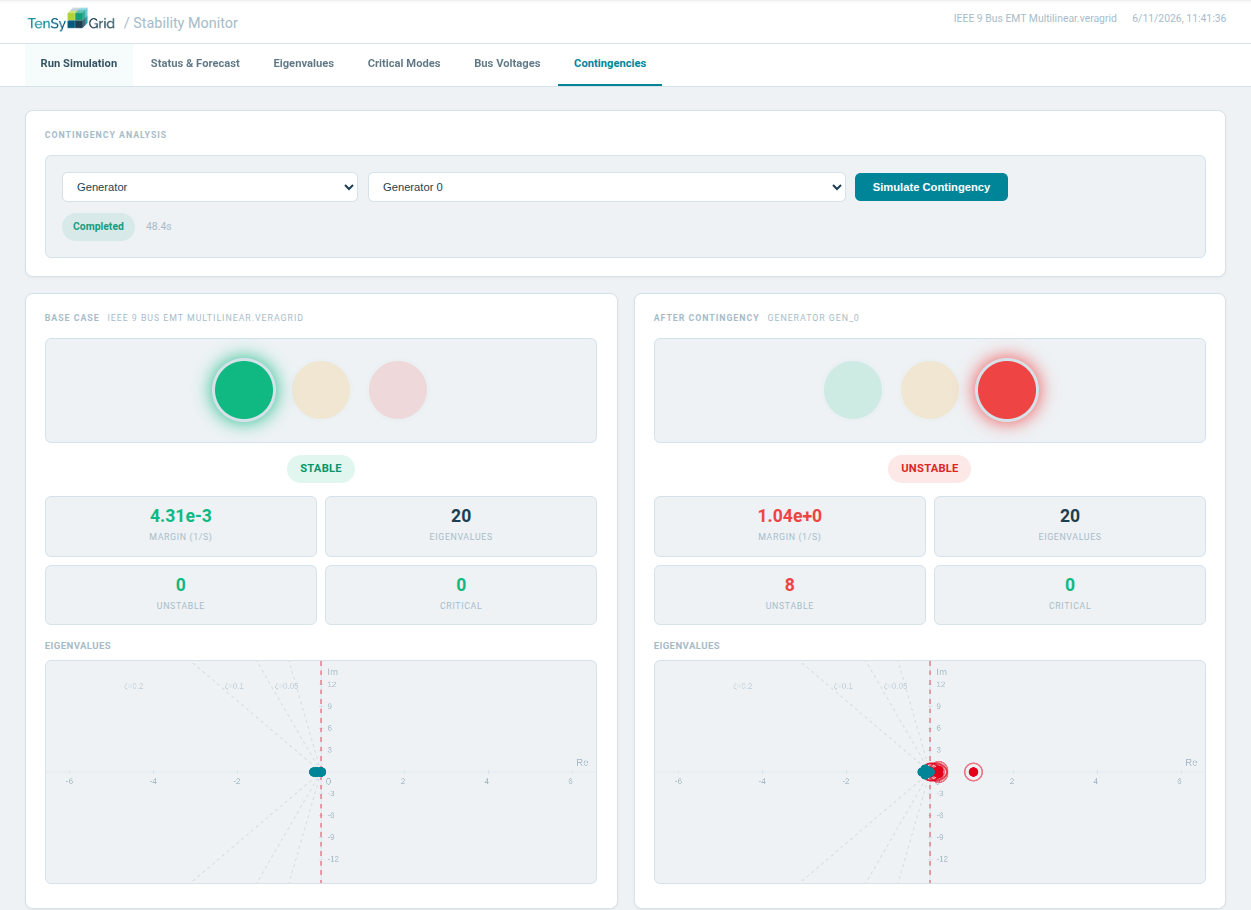
\includegraphics[width=\linewidth,height=0.52\paperheight,keepaspectratio]{assets/generator-outage.png}\\[0.5ex]
      {\scriptsize Source: MS4.1, Fig. 3; base case and generator-outage comparison.}
    \end{column}
    \begin{column}{0.38\textwidth}
      \begin{itemize}\setlength{\itemsep}{2ex}
        \item \textbf{Base case:} stable, no unstable eigenvalues.
        \item \textbf{After the outage:} unstable, with \textbf{8 unstable eigenvalues}.
        \item Compare the spectra, then inspect the critical modes to investigate the change.
      \end{itemize}
    \end{column}
  \end{columns}
\end{frame}

% 8 -- 1:00. Concurrent hackathon confirmed by Alexandre.
% Sources: hackathon/participant_challenge.tex (draft participant brief)
% and hackathon/hackathon_schedule.tex (programme).
% Omit draft scoring weights and differing scenario counts across the sources.
% No participants, awards or lessons are reported before the event finishes.
\begin{frame}[t]{Hackathon -- Keep the grid stable}
  \framesubtitle{Hands-on use of VeraGrid and the TenSyGrid analysis tools}
  \vspace{1.5ex}
  Keep the grid stable while minimising losses, damping oscillations and limiting structural changes. Participants will be given a network model and a set of operating scenarios. They will be asked to:
  \par\vspace{2ex}
  \begin{columns}[T,onlytextwidth]
    \begin{column}{0.31\textwidth}
      {\color{tgpetrol}\large\textbf{Lower losses}}\\[0.5ex]
      Optimise topology and dispatch.
    \end{column}
    \begin{column}{0.33\textwidth}
      {\color{tgpetrol}\large\textbf{Better damping}}\\[0.5ex]
      Tune controls to maintain stability.
    \end{column}
    \begin{column}{0.30\textwidth}
      {\color{tgpetrol}\large\textbf{Fewer changes}}\\[0.5ex]
      Limit structural interventions.
    \end{column}
  \end{columns}
  \par\vspace{3ex}
  \centering
  \begin{tikzpicture}[
    hackstep/.style={draw=tgpetrol, fill=tgpetrol!7, line width=0.6pt,
        text width=2.85cm, minimum height=1.3cm, align=center,
        inner sep=4pt, font=\small},
    flow/.style={-{Latex[length=2mm]}, draw=tgpetrol, line width=1pt}
    ]
    \node[hackstep] (warmup) at (0,0) {
      \textbf{1. Reconstruct}\\[0.5ex]
      From $S$, $\Phi$ to a\\Python function
    };
    \node[hackstep] (optimise) at (3.55,0) {
      \textbf{2. Optimise}\\[0.5ex]
      Baseline, topology\\and dispatch
    };
    \node[hackstep] (tune) at (7.1,0) {
      \textbf{3. Stabilise}\\[0.5ex]
      Eigenvalues and\\converter tuning
    };
    \node[hackstep] (test) at (10.65,0) {
      \textbf{4. Automate \& test}\\[0.5ex]
      Repeat across\\operating scenarios
    };
    \draw[flow] (warmup.east) -- (optimise.west);
    \draw[flow] (optimise.east) -- (tune.west);
    \draw[flow] (tune.east) -- (test.west);
  \end{tikzpicture}
  \par\vspace{2ex}
  \raggedright
  \textbf{Team output:} a runnable strategy and a short explanation of the approach.
  \par\vspace{1ex}
  {\color{tgpetrol}\textbf{For WP4:} exercise the workflow and gather feedback on usability and documentation.}
\end{frame}

% 9 -- 2:00. Sources: D4.1 sections 3.3 and 4; MS4.1 further development.
% Prioritisation proposals, not commitments to implement all nine extensions.
% Nonlinear methods, particularly region of attraction, remain exploratory.
\begin{frame}[t]{Next steps and priorities}
  \vspace{1ex}
  \begin{itemize}\setlength{\itemsep}{1.8ex}
    \item \textbf{Select extensions:} prioritise scenario comparison, critical-element ranking and reporting according to user value and feasibility.
    \item \textbf{Expand validation:} test different network sizes and generation mixes, with reference comparisons.
    \item \textbf{Consolidate the toolbox:} improve error diagnostics, usability and documentation.
    \item \textbf{Agree the implementation scope:} define partner contributions and investigate the feasibility of nonlinear methods.
  \end{itemize}
  \vfill
  {\color{tgpetrol}\textbf{The catalogue guides selection; proposed cases are not implementation commitments.}}
\end{frame}

% 10 -- Funding acknowledgement, kept from the supplied template.
% Funding logos and legal wording also appear on the title slide.
\begingroup
\setbeamertemplate{footline}{}
\begin{frame}[c]{Acknowledgement}
  \small
  \insertack
  \vspace*{3ex}
  % Keep the template's logo rows within the available text width.
  \compactfundinglogos
\end{frame}
\endgroup

\end{document}
